\section{Design of the Solution}

\label{sec:design}
%missing introduction?

\subsection{Assumptions}

% A table 

Building a model always depends on assuming certain assumptions. The generalisations taken in the 
assumptions allows one to focus on the global mechanics and do not take corner cases into account. 
As exceptions, they are part of the reality but they do not have material importance to change the result 
of the model.

The design of the AppCoins platform was made having the following eight assumptions:

\begin{itemize}
\item {\bf\em A1 Crowdsourcing}: Community wisdom works for big numbers better than individual 
wisdom \cite{Surowiecki:2005:WC:1095645};
\item {\bf\em A2 Incentives}: If there are enough incentives, community contributes;
\item {\bf\em A3 New}: A new developer is always an unknown developer;
\item {\bf\em A4 Trusted:} The Apps from a Trusted Developer are Trusted Apps;
%chose between how to use capitals: Developer vs developer in A3 and A4
\item {\bf\em A5 Dispute}: - In a dispute, if 50\% + 1 of the community is honest, the right side wins;
\item {\bf\em A6 Reputation}: - Transactions registered in the blockchain ledger (IAB, Ads) reflects well 
the trustworthiness and reputation of a developer;
\item {\bf\em A7 Unknown downloads}: - If the app downloads made by the users come from more than 
5\% of unknown developers, users will start to have trust in unknown developers.
\item {\bf\em A8 Zero-day}: - A community dispute may take 30 days. While the dispute is handled, the 
app stores have the option to hide the app to avoid zero-day attacks.
\end{itemize}



\subsection{Client side support}

Besides the blockchain technology, the environment where the user is running the app store should 
also support the AppCoins protocol.

% TODO }: include quote
%missing context and connection to previous sentence?

As Android represents 86\% of the smartphones market, we focus an implementation analysis in that 
platform. However, many of the constraints and solutions are applicable to other smartphone operating systems.

This subsection\footnote{This section was contributed by Marcelo Benites, Aptoide Android team 
member} aims to describe a client-side method, running in the smartphone's untrusted environment, to 
register that a user is paying attention to an app (installed from an app store) for a certain amount of time. Once those requirements are met, a \textit{proof-of-attention} (\textsf{PoA}) is requested and stored in the 
blockchain.
 
%XXX describe what is a proof-of-attention
 
Concepts definition: %improve this introductory sentence?
\begin{itemize}
\item {\bf App store}: PoA compliant app store Android app.
\item {\bf Application}: Android app installed from the app store.
\item {\bf User}: user registered in the app store.
\end{itemize}

When designing a solution, two main factors should be taken into account: reliability and availability. 
Reliability consists in avoiding fraud. Once a \textsf{PoA} is generated, it has to have a high level of 
confidence that a user paid attention to an app installed from an app store. Availability consists in 
making sure that whenever a user pays attention to an app installed from an app store, the app store 
will be aware of that and will request the \textsf{PoA} once the requirements are met. %requirements?

The app store process has to be running when the user is paying attention to an app in order to request  
the \textsf{PoA}. Latest releases of the Android operating system (Android OS) - from Lollipop (API 
level 21) onwards - have been limiting the ability of app processes to run while the app is in the 
background. In our scenario the app store process could eventually be killed by the Android OS while 
not being in the foreground. In order to overcome that issue, we will take advantage of the Binder 
framework to bind the app and app store's processes while the app is in the foreground, which will 
ensure that the app store process is not killed by the Android OS. 

\begin{figure}[!ht]
\centering
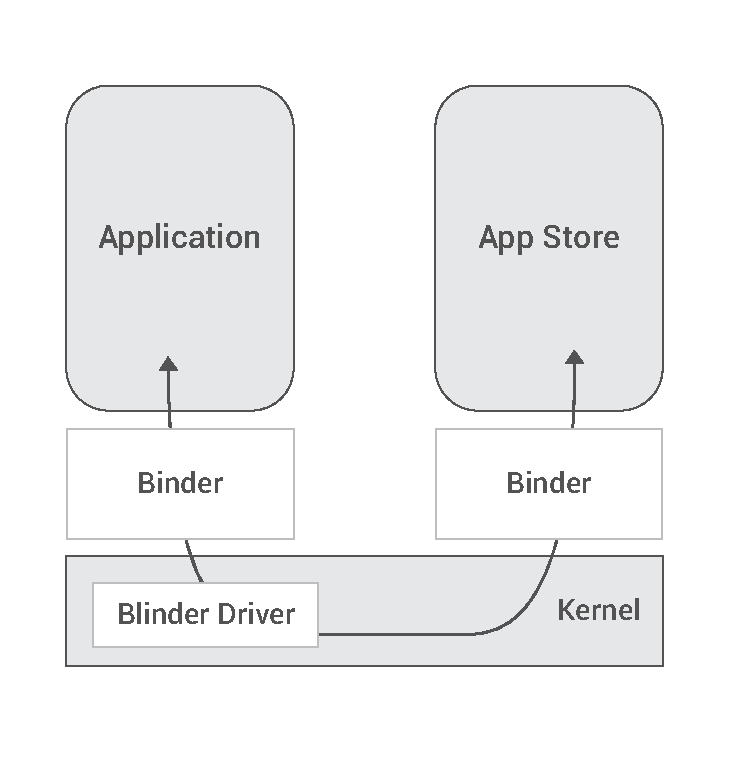
\includegraphics[width=0.5\textwidth]{diagrams/binder_diagram.eps}
\caption{Operating system binder.}
\label{fig:binder}
\end{figure}

Binder framework is a core component in Android architecture and its main goal is to simplify Inter-
Process Communication (IPC). Binder is implicitly used whenever an app communicates with OS 
services or with other apps through the Android Java API Framework. The Binder framework will also 
provide information regarding the app process, which will positively contribute to the app store 
\textsf{PoA} reliability.

Once the app and the app store's processes are bound, the app store will periodically verify whether 
the app is in the foreground and the user is actively interacting with the device. In order to certify that 
the user is paying attention to the app, the following conditions should be met:
%are conditions the same as what was previously called requirements?

\begin{itemize}
\item The app's process must be bound to the app store's process.
\item The app must be in foreground.
\item The device screen must be on.
\item The device must not be locked. 
\item The signature of the app must be verified on the app store's servers.
\end{itemize}

To assure that the app's process is bound to app store, Binder and PackageManager APIs can be used. 
To verify whether an app process is in the foreground, both ActivityManager, UserStatsManager and 
%or?
 PackageManager APIs can be used. To check whether the device screen is on, the PowerManager 
and Display APIs can be used. Regarding the state of the lock screen, the KeyguardManager API can 
be used. 

Every application has to be signed by the developer before being installed on an Android device. App 
stores have access to the apps' signatures and can validate by confirming whether they match with the 
signature on their servers. If the signature does not match, the app may have been tampered with. To obtain the app's signature, the Binder and PackageManager APIs can be used.

\subsubsection{Limitations client-side}

The proposed solution has some limitations regarding reliability - imposed by Android's inherently 
insecure environment - and Android API availability - due to Android's version fragmentation and app 
store permission level. The use of several different Android APIs can help harden the solution 
against an attacker but can not assure full protection against fraud on the client side. In order to 
mitigate fraud, a system has to have different security layers both on the client side and the server side. 

In Android some APIs are considered sensitive and require system-level permissions to access them. 
Usually system-level can only be granted to system applications (pre-installed on the device by 
manufacturers). Also some APIs are only available in certain versions of Android. Table \ref{table: permissions} summarises the APIs needed to generate the \textsf{PoA} and their availability:

\begin{table}[H]
\scriptsize
\centering
\begin{tabular}{|l|l|l|l|l|l|}
\hline
\textbf{API Class}                          & \textbf{API Method}                  & \textbf{Min API}      & \textbf{Max API}       & \textbf{Permission Level}               & \textbf{Permission}                             \\ \hline
\multirow{2}{*}{PowerManager}      & isScreenOn                  & API 7       & API 19       & \multirow{2}{*}{None}          & \multirow{2}{*}{None}                  \\ \cline{2-4}
                                   & isInteractive               & API 20      & None                  &                                &                                        \\ \hline
Display                            & getState                    & API 20      & None                  & None                           & None                                   \\ \hline
Binder                             & getCallingUid               & API 1      & None                  & None                           & None                                   \\ \hline
\multirow{2}{*}{ActivityManager}   & getRunningAppProcesses      & API 3      & API 21     & None                           & None                                   \\ \cline{2-6}
                                   & getRunningTasks             & API 1      & API 20       & Normal-Level                   & GET\_TASKS                             \\ \hline
\multirow{2}{*}{PackageManager}    & getPackagesForUid           & API 1      & \multirow{2}{*}{None} & \multirow{2}{*}{None}          & \multirow{2}{*}{None}                  \\ \cline{2-3}
                                   & getPackageInfo              & API 1      &                       &                                &                                        \\ \hline
\multirow{2}{*}{KeyguardManager}   & isKeyguardLocked            & API 16  & \multirow{2}{*}{None} & \multirow{2}{*}{None}          & \multirow{2}{*}{None}                  \\ \cline{2-3}
                                   & isDeviceLocked              & API 23 &                       &                                &                                        \\ \hline
\multirow{2}{*}{UsageStatsManager} & isAppInactive               & API 23 & None                  & \multirow{2}{*}{System-Level} & \multirow{2}{*}{PACKAGE\_USAGE\_STATS} \\ \cline{2-4}
                                   & queryAndAggregateUsageStats & API 21    & None                  &                                &                                        \\ \hline
\end{tabular}
\caption{\textsf{PoA} generation Android APIs. The \textit{UsageStatsManager} requires a System-Level permission but the PACKAGE\_USAGE\_STATS can also be obtained by a normal application if the user explicitly enables it in the Settings.}
\label{table: permissions}
\end{table}


%\begin{figure}[!ht]
%\centering
%\includegraphics[width=\textwidth]{diagrams/table_android_limitations.eps}
%\caption{Table of Android versions and API support}
%\label{fig:android_versions}
%\end{figure}



We can only have an implementation that fulfils all the requirements to certify that the user is paying 
attention to the app with a minimum Android version of Jelly Bean (API 16) and above. The Android 
version limitation is not relevant since according to Google statistics, only 1.2\% of the Android devices are not running version Jelly Bean (API 16) or above. %reference missing

Also, UsageStatsManager is necessary from Lollipop (API 21) onwards requiring that, either the app 
store app is a system app, or asking the user to explicitly go to Settings and give the permission. Since 
in the App Economy the user will be rewarded by the attention given to apps, it will be easy to convince 
him to manually provide the permission in the case where the app store is not a system application.


\subsection{Protocol Overview and sketch}


The AppCoins protocol is depicted in Figure \ref{fig:design}. It consists in 3 main blocks: Advertising, 
Developer's Reputation (Rank) and IAB.

\begin{figure}[!ht]
\centering
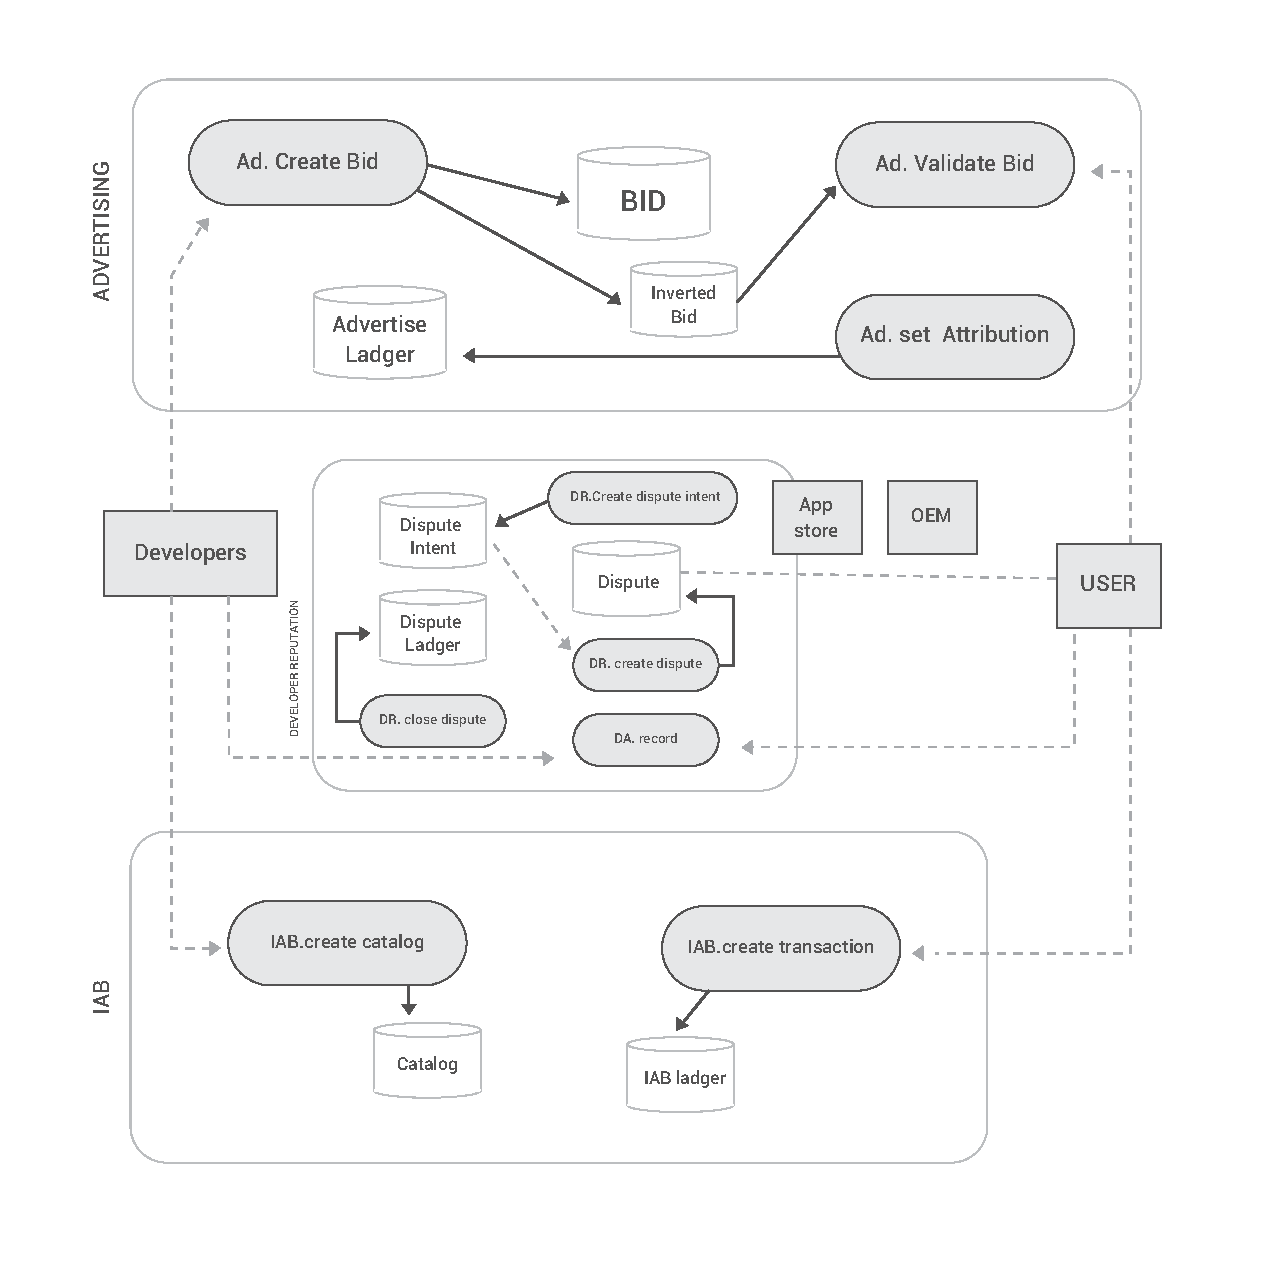
\includegraphics[width=0.8\textwidth]{diagrams/design.eps}
\caption{Overall design of AppCoins and blockchain interactions.}
\label{fig:design}
\end{figure}

Inside each block we see the interactions between the ecosystem players and the blockchain. The 
rounded squares represent functions / methods of smart contracts that implement business logic. The 
cylinders represent data stored in smart contracts' own storage or event logs. \\

{\bf Advertising}

The protocol was defined such that most risks in Section \ref{subsec:intro_ads} are avoided or at least mitigated. By leveraging blockchain technology and its requirements of transparency, accountability and verifiability of processes, we avoid creating a middlemen-dependent economy and add value both for the advertisers/developers and the users. \\

As explained in Section \ref{sec: introduction}, there are three moments in an advertising model: campaign creation, impression and attribution (which can be an installation, opening of the app, etc).  In AppCoins protocol, an attribution does not happen when the user installs the app or game, but after the app is opened for 2 minutes. This poses the problem of how can the app store prove that a user did indeed open the app and had it opened for the required period of time. Our protocol introduces a \textit{proof-of-attention} \textsf{PoA}, which allows the developers to verify that users did actually paid attention to the app for the required time. \\

Since the smartphone is an untrusted environment, there is not a total guarantee that the user is real or that the app store stub installed in the phone was not tampered. However, identity is checked server side by the app store using network fingerprint (IP, routing information, etc) as it is done today by the tracking platforms. Similar challenges to \textsf{PoA} are addressed in BAT \cite{BAT}. \\

From the requirement of privacy, the protocol itself does not expose any user information at any time and interaction with app stores. The only information that can be seen by others are the wallet addresses when a transaction occurs. Concerning risk \textsf{R1.4}, since the addresses are not linked to any sensitive user information (e.g. email), there is no leakage of user data. \\

Regarding risk \textsf{R1.6}, developers can claim that a certain user did not actually do the required action to be given the attribution, i.e. that either the app store, the user or both are being dishonest. By providing a \textsf{PoA} and storing the transactions in the blockchain, they become verifiable by anyone, including the developer. Since the developer can verify the proof, it becomes clear that the protocol avoids the risk of repudiation. \\

Since our solution proposes that no middlemen is needed within the advertising model, there is the need to have the protocol being able to enforce the payments between the developer and the other parties, which are the user, the app store and the OEM. The only way to make sure the entirety of the funds that the developer wants to put available for the campaign exist is to lock them in a different wallet, which is where the smart contract for the campaign will be running. Since they are locked, the developer cannot spend them before the campaign is over and there is no possibility for the developer to be in default. In addition, when there is an impression, the amount of tokens to be paid for that conversion need to be locked as well. This serves to avoid race conditions, which can occur when the funds still available in the campaign are for $X$ attributions but $Y$ users are getting impressions for the campaign (with $X < Y$). If this would be possible, some of the $X$ users would install the app but when they opened it and paid attention to it for the required time, thus being eligible for the attribution, they would not get the attributed because there would be no more funds available. This means that different wallets need to exist that serve to lock funds for the already made impressions. If the attribution for a certain impression does not occur after some designated amount of time, then the funds would be unlocked and placed back in the campaign wallet. This funds captivation scheme is exemplified in Figure \ref{fig:wallet_cpi_flow} and avoids the risk \textsf{R1.5}.\\

{\bf IAB}

The IAB use case has the risks outlined in Section \ref{subsec:intro_iab}, which the protocol needs to either avoid or mitigate. \\

As in the Advertising use case, since the protocol follows the requirements of blockchain technology, and in particular the requirement of privacy, the protocol only exposes wallet addresses when transactions occur. These need to be publicly available in order to have the possibility of verifying transactions but do not carry any link to personal user information (for example, the email of the user). Therefore, risk \textsf{R2.1} is partially avoided. \\

The protocol is built to allow for transparency between users, developers and app stores. Transparency means that transactions between parties are public and verifiable, but only regarding token exchange. This means that the protocol is not intended to store items or any other form of goods/value. This tracking, as it is today, is to be done directly by users and developers, i.e. when the user pays for an in-app item, it is the user's responsibility to check if the item is transferred or not. The store, retrieve, and exchange of digital items between users is out of the scope of the AppCoins solution. Nonetheless, having the transactions publicly available mitigates this problem, which is referred to as risk \textsf{R2.2}, but does not completely avoid it. However, because of having the transactions publicly available, the protocol avoids risk \textsf{R2.3} because the user only sends more tokens in exchange for an in-app item if wanted. \\

Regarding item cloning, as it has been said, the protocol itself does not deal with in-app items or their exchange, only with the token transfers in the scope of in-app purchases. Hence, there is no possibility within the protocol to clone items and neither to send them to other users. Therefore, risk \textsf{R2.4} is not addressed by the protocol at this version.\\


{\bf Developer Reputation}

This use case is the one that may dictate if a developer is trustable or not. Therefore, if the protocol defines ways to mitigate and avoid malware attacks across the app stores operating within the protocol, then the adoption of the protocol by app stores can be greatly increased. \\

As it was said in Section \ref{subsec:intro_approval}, the malware scanning process is different for all the app stores, as are the reasons for blacklisting apps. An app store that is not showing an app to its users because it is from a competitor or for censorship purposes, although the app was considered ``trusted'' in the blockchain, is then exposed in the community. If the malware knowledge is not shared across app stores - the current state - will fin act harm users because one app with malware may have already been blacklisted in an app store but it still available on others. Our protocol deals with this problem by attributing a reputation level to the developers, which is then extended to all their apps. \\

The reputation of a developer has two components: the rank and the rank level. The rank can have the values of \textit{"Unknown"}, \textit{"Trusted"} or \textit{"Critical"} and it states if a developer is new to the community, if it is already known and considered honest or if it is considered dishonest, respectively. The rank level is represented by an integer starting at 1 and does not have a maximum level for the \textit{"Trusted"} rank. However, for the other ranks it is fixed at 1. This derives from the fact that when a developer is \textit{"Unknown"}, it is just because the developer is new in the network and the goal is that the developer leaves the rank to become \textit{"Trusted"}. On the other hand, being a \textit{"Critical"} developer means the developer is dishonest and we do not intent to have different levels of dishonesty in the network. Figure \ref{fig:approval_state_diagram} shows the different ranks a developer can have and how to move from one rank to another. \\

\begin{figure}[!ht]
\centering
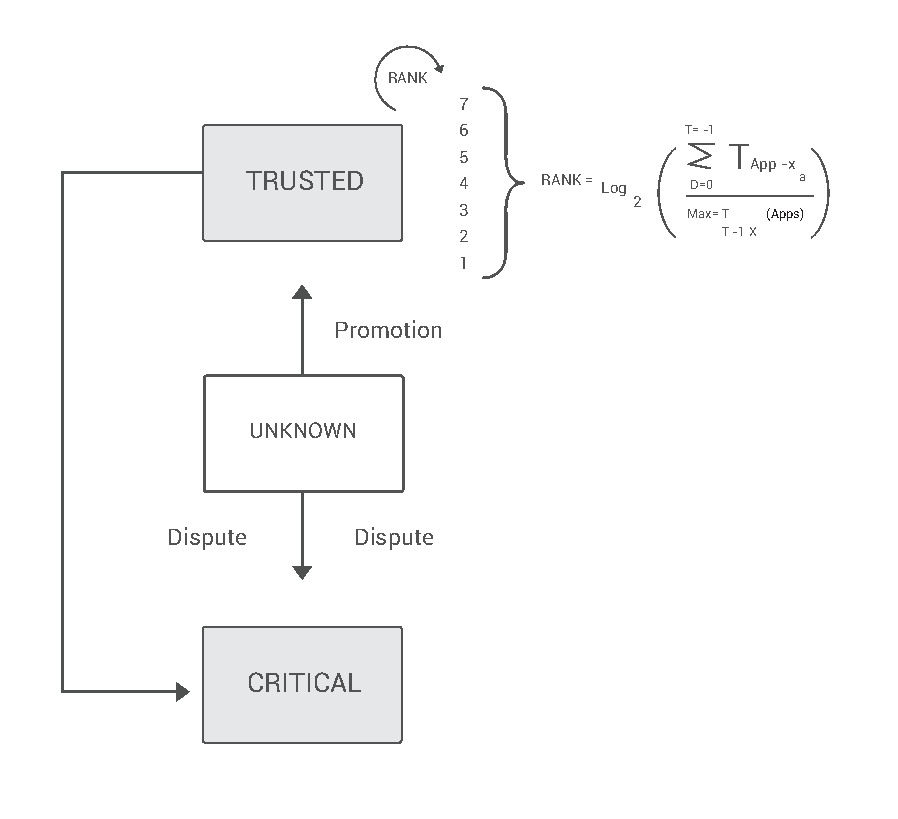
\includegraphics[width=0.5\textwidth]{diagrams/approval_state_diagram.eps}
\caption{Approval state changes.}
\label{fig:approval_state_diagram}
\end{figure}

As it can be seen, there are two processes by which the rank can change: \textit{promotion} and \textit{dispute}. A \textit{promotion} is an automated process which takes into account the number of transactions occurred in the developer's apps and compares them to the transactions of other popular apps from trusted developers. If the developer's apps compare well against others (this comparison is detailed in Section \ref{subsec:protocol_devrank}), the rank is either increased to \textit{"Trusted"} or the rank level goes up one level in the case where the developer is already \textit{"Trusted"}. \\

Regarding the \textit{dispute}, it is a mechanism to punish developers that deliver bad apps, either because they contain malware or they are fake, i.e. do not do anything and may contain only ads. This process of judging developers has been a centralised process in app stores and our protocol introduces a way to have it done by the community, since it is the community that uses the apps. The protocol provides a way to open a dispute against a developer, i.e. any user can claim that a developer is dishonest. When a dispute is started, which at this point we call as a \textit{dispute intent}, any user can answer it within the next 7 days. The user answering it, which would mean that the user is claiming the developer is honest, can be any user and does not need to be the developer. If the dispute intent is answered, a dispute is opened and stays open for 30 days. Within this time period, any user can join any side of the dispute, either the \textit{Contestants} - users who claim that the developer is dishonest - or the \textit{Pleaders} - users who claim the developer is in fact honest. If the dispute intent is not answered by anyone, the dispute intent is closed without opening a dispute and the developer's rank changes to \textit{"Critical"} along with the rank of all the apps of that developer. \\

In order to join a dispute, a user needs to put an amount of tokens into stake. The amount of tokens is chosen by the user and express the confidence in the side the user is joining. When the 30 days of the dispute are over, the side which collected the biggest amount of tokens wins. The winning side gets a refund of the tokens pledged plus 10\% of the pledge of the losing side. This 10\% is divided according to the percentage each user had pledged within the winning side pledge. The losing side gets a refund, where the pledge of each user has a cut of 10\%. Regarding the change in the developer's rank, if the \textit{Contestants} win, the developer's rank changes to \textit{"Critical"} and all the apps of the developer also have their rank changed. On the other hand, if the \textit{Pleaders} win, the developer's rank remains unchanged. \\

The dispute mechanism transfers power back to the community, which can also include the app stores. Since it is the community deciding whether a developer and the corresponding apps are to trusted or not, the developers reputation and the reasons for it are public to everyone. If there is a change in the reputation of a developer, the community knows when it happened and knows it was a decision made by them, instead of being obscurely made by one app store. This mitigates the risks \textsf{R3.3} and \textsf{R3.4}. \\

Risk \textsf{R3.2} is similar to risks \textsf{R1.4} and \textsf{R2.1} and the reason why it is avoided by the protocol is the same.


% a diagram that integrates all the players
% the circular but more geek 

%(Include a diagram with the players - component diagram 

% Could be a sequence diagram as in Filecoin diagram 

% (In-App Billing, Advertising, Reputation builder) 

%


